\section{Pilotforsøg}
I dette bilag beskrives, hvorledes pilotforsøget udføres.
%TAGER VI TIL SIDST

\subsection{Formål}
Dette pilotforsøg har til formål at kunne præcisere samt optimere kravspecifikationerne i de enkelte blokke, hvorved uklare parametre forventes at kunne besvares. Disse parametre omfatter identificering af støj signaler, EMG-signalets frekvensområde samt elektrodernes placering. Parametrene vil forsøges besvaret udfra målinger ved udførelse af en squat-øvelse.
Hertil anvendes en EMG-forstærker og et accelerometer som sensorer. På baggrund af dette opstilles følgende formål for de enkelte sensorer.  

\subsubsection{EMG-forstærker}
\begin{enumerate}
\item Opsamling af signal fra rectus femoris og biceps femoris
\begin{itemize}
\item Identificering af elektrodernes placering
\item Sammenligning af muskelaktivitet oprejst og i en squat-øvelse 
\end{itemize}
\item Identificering af støjsignaler
\item Identificering af frekvensområde
\item Identificering af gain til mikroprocesserens operationsspænding
\end{enumerate}

\subsubsection{Accelerometer}
\begin{enumerate}
\item Identificering af knæleddets position siddende i en squat-øvelse
\item Identificering af støjsignaler
\end{enumerate}

\subsection{Materialer} 
\begin{itemize}
\item EMG-forstærker
\item Elektroder %Hvilke elektroder?
\item Desinfektionsservietter
\item Skraber
\item Tusch 
\item Accelerometer ADXL335Z
\item Tape
\item Ledninger %Hvilke ledninger?
\item Computer
\item CY8CKIT-042-BLE
\end{itemize}

\subsection{Metode}
For at identificere den bedst mulige elektrodeplacering tages der udgangspunkt i den anatomiske afbildning af låret, som ses af \autoref{fig:laarmuskler}.

\begin{figure}[H]
\centering
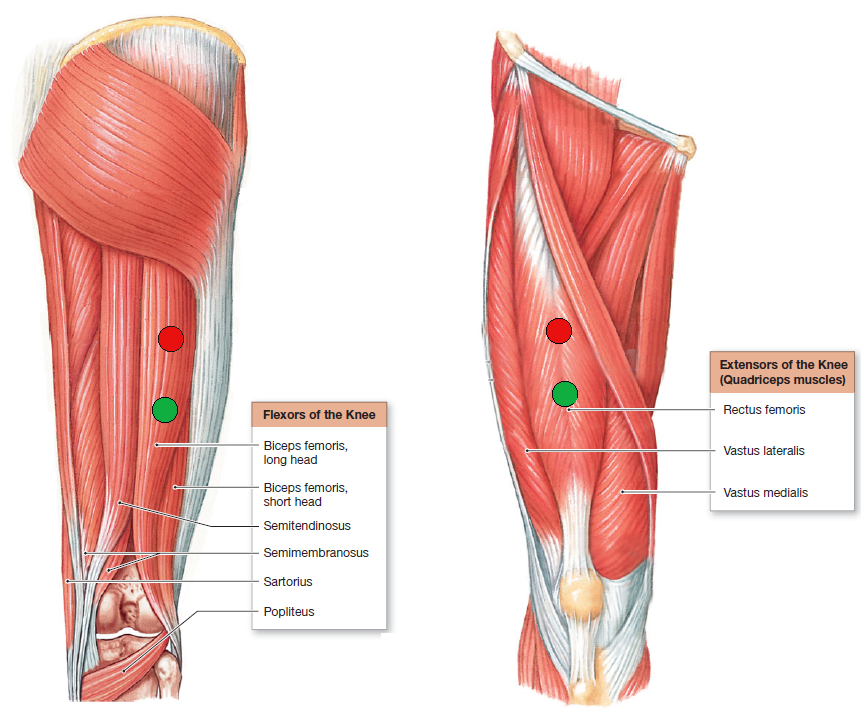
\includegraphics[width=0.5\textwidth]{figures/laarmuskler.png}
\caption{BILLEDTEKST \citep{martini2012}.}
\label{fig:laarmuskler}
\end{figure}

Elektroderne placeres medialt for både rectus femoris samt biceps femoris for så vidt muligt, at elektroderne forbliver over musklen ved en kontraktion. 

Da der ikke fremgår nogen muskel på den superiore mediale del af tibia, benyttes dette som referencepunkt for EMG-målingen, hvortil der forventes en stabil reference. 

 %Det skal beskrives hvad der tages udgangspunkt i for placering af elektroderne (anatomisk placering af muskel og hvor på musklen.) evt billede.. Referencepunkt??




For at identificere støj fra EMG-forstærkeren fortages der baselinemålinger.
%optages aktivitet i musklerne i en squat-øvelse. 


For at simulere den påvirkning som accelerometeret udsættes for og derved identificere det maksimale og minimale outputsignal roteres accelerometeret i en langsom rotation fra 0$^{\circ}$ til 90$^{\circ}$ både til højre og venstre. Herudover måles accelerometerets påvirkning i henholdsvis 0 og 1 g-påvirkning for at identificere accelerometeres påvirkning samt, hvorvidt dette stemmer overens med databladet. 
% 'For at' i starten af hver sætning - væk!

\subsection{Forsøgsopstilling}
Forsøgsopstilling er for den primære udførelse af forsøget. Nogle af processerne gentages for at kunne sammenligne de forskellige målinger, og derved få et bedre resultat.
% Omskriv..

\subsubsection{EMG-forstæker}
Rectus femoris og biceps femoris identificeres, den ønskede placering af elektroderne markeres med tusch. Herefter fjernes eventuelle hår og døde hudceller ved brug af skraber. Huden desinficeres herefter ved brug af desinficeringsservietter og elektroderne påsættes. Den røde ledning påsættes rectus femoris/bicep femoris og den grønne ledning påsættes rectus femoris/bicep femoris. Den sorte ledning påsættes patella og anvendes som referencepunkt.
% Benyttes der en eller to emg forstærkere??? I givet fald skal det beskrives mere tydeligt.

\subsubsection{Accelerometer}
Accelerometeret placeres lateralt på låret, således accelerometeret måles i xyz-plan, hvorved der måles i den vertikale retning. Der sørges for, at accelerometeret befinder sig i 0 g-påvirkning ved starten af forsøgets udførelse, hvorved accelerometeret er kaliberet. 

\subsubsection{Opstilling}
\begin{itemize}
\item Identificering af musklerne rectus femoris og biceps femoris 
\item Elektrodernes placering markeres
\item Huden skrabes og desinficeres
\item Elektroderne påsættes
\item Ledningerne påsættes elektroderne
\begin{itemize}
\item Den røde/grønne ledning på rectus femoris
\item Den røde/grønne ledning på biceps femoris
\item Den sorte ledning/reference på patella \fxnote{positiv/negativ/ground}

\end{itemize} 
\item Accelerometeret påsættes patella ved en 0 g-påvirkning i xyz-retning
\end{itemize}
% ikke patella

\subsection{Fremgangsmåde}
Fremgangsmåden udføres XX antal gange, hvorved der på baggrund af målingerne foretages en gennemsnitsværdiberegning.
%Bruges til hvad?

\subsubsection{EMG/EMG-forstærker}
EMG-måling: 10-sekunders målinger trinvist under udførelse af en squat-øvelse. 


\subsubsection{Accelerometer}
Påvirkning i 0 og 90$^{\circ}$.
Påvirkning af rotation fra 0 til 90$^{\circ}$ både til højre og venstre.
Optag 30 sekunder ved 0 og 90$^{\circ}$ .
Optag rotation: baseline 10 sekunder, rotation 10 sekunder, baseline 10 sekunder

%sampling - optag


